\documentclass[a4paper, 12pt]{article}

\usepackage{tikz} % main tikz package

\usetikzlibrary{external}
\tikzexternalize[prefix=compiled_figures] % prefix sets where to store figures

% for a nicer colorscheme
\definecolor{blue}{rgb}{0.38, 0.51, 0.71} %glaucous, 97,130,181, #6182B5
\definecolor{darkblue}{RGB}{17, 42, 60} % 112A3C
\definecolor{red}{RGB}{175, 49, 39} % AF3127

\definecolor{orange}{RGB}{217, 156, 55} % D99C37
\definecolor{green}{RGB}{144, 169, 84} % 90A954
\definecolor{palegreen}{RGB}{197, 184, 104} % C5B868

\definecolor{yellow}{RGB}{250, 199, 100} % FAC764
\definecolor{brokenwhite}{RGB}{218, 192, 166} % DAC0A6
\definecolor{brokengrey}{rgb}{0.77, 0.76, 0.82} % {196,194,209}, C4C2D1


\begin{document}
    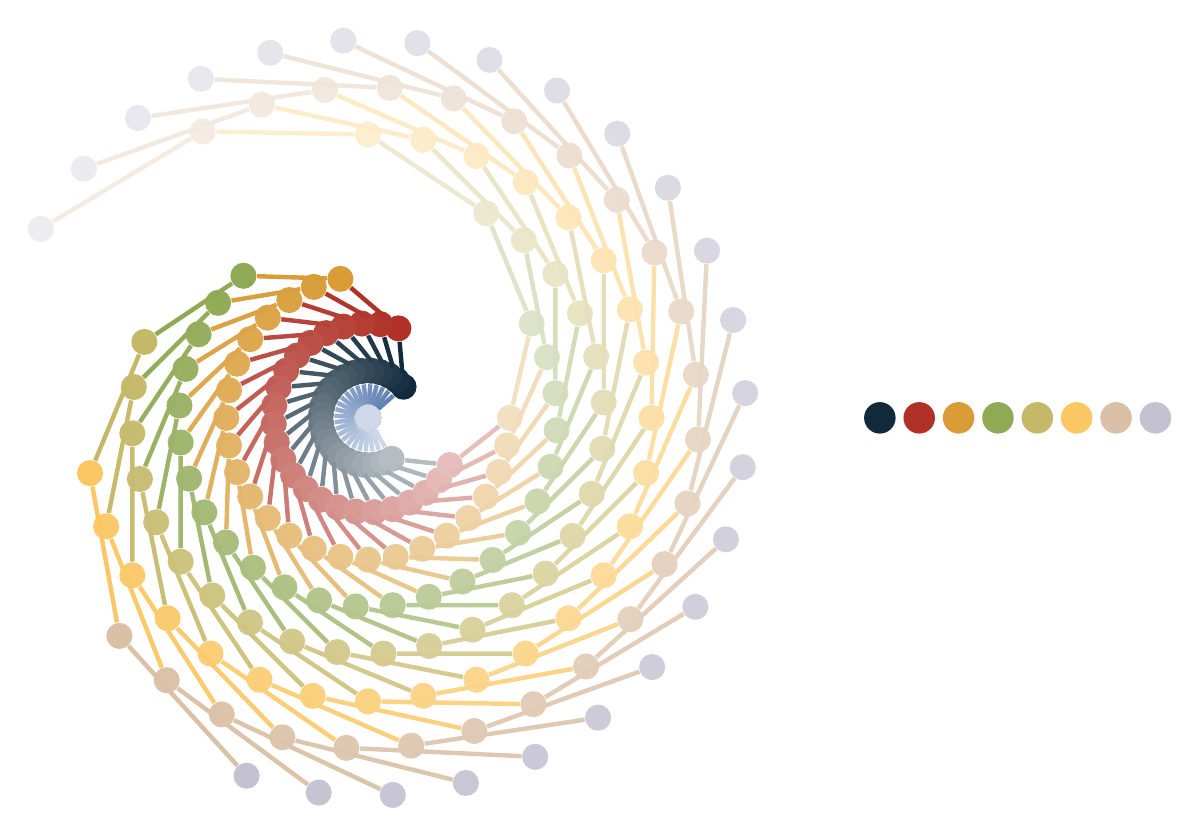
\begin{tikzpicture}

        % the following is equivalent to defining \col as a counter (see the next loop)
        % but this showcases zipped loops
        \foreach \color / \col in {
                        blue/0, darkblue/1, red/2, orange/3, green/4,
                        palegreen/5, yellow/6, brokenwhite/7, brokengrey/8} {
            \foreach \alpha [count=\row] in {100, 97, ..., 30} {
                % the step (-3) of the loop is infered from the two first values

                % random formula to define an angle for the current point and radius
                \def \angle {180*\row/16 + 30*\col};
                \def \radius {0.6*\col};

                % define a coordinate (center\color\alpha) (which are expanded to their actual
                % value so that we can draw a node it later, and have line from the border
                \coordinate (center\color\alpha) at ({\radius*cos(\angle}, {\radius * sin(\angle)});

                % draw a filled circle node named (circle\color\alpha) centered
                % at (center\color\alpha)
                % we define a new node so that lines will leave from the edge of
                % the circle and not from its center
                \node[circle, fill=\color!\alpha] (circle\color\alpha) at (center\color\alpha) {};

                % make a nice line (to showcase an if)
                \ifnum \col = \row
                    \fill[color=\color, xshift=6cm] (0.5*\col, 0) circle (0.2);
                \fi
            }
        }

        % this showcases a trick to iterate on couples (i-1,i) using the remember keyword
        \foreach \color[remember=\color as \lastcolor (initially blue)] in
                        {darkblue, red, orange, green, palegreen,
                        yellow, brokenwhite, brokengrey} {
            \foreach \alpha in {100, 97, ..., 30} {
                \draw[ultra thick, color=\lastcolor!\alpha] (circle\lastcolor\alpha) -- (circle\color\alpha); 
            }
        }
    \end{tikzpicture}

    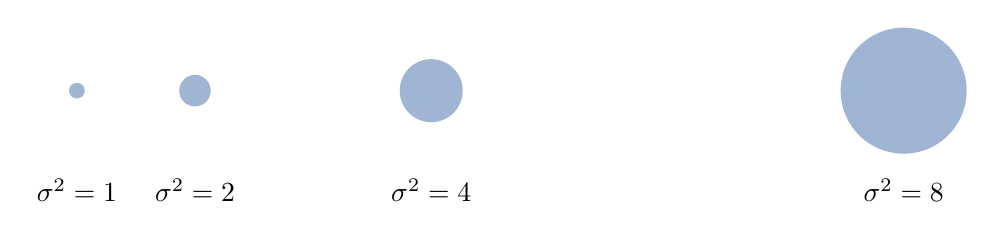
\begin{tikzpicture}
        \def \mathvariable {\sigma^2};
        \def \colorvariable {blue};
        \def \alphatransparency {60};
        \def \basewidth {0.1cm};

        % iterate on the list {1,2,4,8}
        \foreach \x in {1,2,4,8} {
            % draw a circle at coordinate (1.5*x, 0) whose radius is x*basewidth
            % use the defined color and transparency
            \fill[\colorvariable!\alphatransparency] (1.5*\x, 0) circle (\x * \basewidth)
                                                    node[below=1cm, black] {$\mathvariable = \x$} ;
        }
    \end{tikzpicture}
    
\end{document}
